\documentclass[14pt, a4paper]{extarticle}
\usepackage{GOST}
\usepackage{array}
\usepackage{verbatim}
\usepackage[detect-all]{siunitx}
\usepackage{amsmath}
\usepackage{amssymb}
\usepackage[utf8]{inputenc}
\usepackage{hyperref}

\usepackage{ifthen}


\usepackage{tempora}


\makeatletter
\renewcommand\@biblabel[1]{#1.}
\makeatother

% Для листинга кода:
\usepackage{listings}
\lstset{ %
	language=python,                 % выбор языка для подсветки (здесь это С)
	basicstyle=\small\sffamily, % размер и начертание шрифта для подсветки кода
	numbers=left,               % где поставить нумерацию строк (слева\справа)
	numberstyle=\tiny,           % размер шрифта для номеров строк
	stepnumber=1,                   % размер шага между двумя номерами строк
	numbersep=5pt,                % как далеко отстоят номера строк от подсвечиваемого кода
	showspaces=false,            % показывать или нет пробелы специальными отступами
	showstringspaces=false,      % показывать или нет пробелы в строках
	showtabs=false,             % показывать или нет табуляцию в строках
	frame=single,              % рисовать рамку вокруг кода
	tabsize=2,                 % размер табуляции по умолчанию равен 2 пробелам
	captionpos=t,              % позиция заголовка вверху [t] или внизу [b] 
	breaklines=true,           % автоматически переносить строки (да\нет)
	breakatwhitespace=false, % переносить строки только если есть пробел
	escapeinside={\#*}{*)}   % если нужно добавить комментарии в коде
}


%для графиков
\usepackage{pgfplots}
\usepackage{filecontents}
\usetikzlibrary{datavisualization}
\usetikzlibrary{datavisualization.formats.functions}

\begin{document}
	
	\begin{table}[ht]
		\centering
		\begin{tabular}{|c|p{400pt}|} 
			\hline
			\begin{tabular}[c]{@{}c@{}} 
\includegraphics[scale=1]{baum.jpg} \\\end{tabular} &
			\footnotesize\begin{tabular}[c]{@{}c@{}}\textbf{Министерство~науки~и~высшего~образования~Российской~Федерации}\\\textbf{Федеральное~государственное~бюджетное~образовательное~учреждение}\\\textbf{~высшего~образования}\\\textbf{«Московский~государственный~технический~университет}\\\textbf{имени~Н.Э.~Баумана}\\\textbf{(национальный~исследовательский~университет)»}\\\textbf{(МГТУ~им.~Н.Э.~Баумана)}\\\end{tabular}  \\
			\hline
		\end{tabular}
	\end{table}
	\noindent\rule{\textwidth}{4pt}
	\noindent\rule[14pt]{\textwidth}{1pt}
	\hfill 
	\noindent
	\makebox{ФАКУЛЬТЕТ~}%
	\makebox[\textwidth][l]{\underline{~«Информатика и системы управления»~~~~~~~~~~~~~~~~~~~~~~~~~~~~~~~~~}}%
	\\
	\noindent
	\makebox{КАФЕДРА~}%
	\makebox[\textwidth][l]{\underline{~«Программное обеспечение ЭВМ и информационные технологии»~}}%
	
	
	\begin{center}
		\vspace{1.5cm}
		{\bf\huge Отчёт\par}
		{\bf\Large по лабораторной работе № 2\par}
		\vspace{0.7cm}
	\end{center}
	
	
	\noindent
	\makebox{\large{\bf Название:}~~~}
	\makebox[\textwidth][l]{\large\underline{Марковские процессы~~~~~~~~}}
	
	\noindent
	\makebox{\large{\bf Дисциплина:}~~~}
	\makebox[\textwidth][l]{\large\underline{~Моделирование~~~~~~~~~~~~~~~~~~~~~~~~~~}}\\
	
	\vspace{1.5cm}
	\noindent
	\begin{tabular}{l c c c c c}
		Студент      & ~ИУ7-75Б~               & \hspace{2.5cm} & \hspace{2cm}                 & &  Д.В. 
		Сусликов \\\cline{2-2}\cline{4-4} \cline{6-6} 
		\hspace{3cm} & {\footnotesize(Группа)} &                & {\footnotesize(Подпись, дата)} & & {\footnotesize(И.О. Фамилия)}
	\end{tabular}
	
	\noindent
	\begin{tabular}{l c c c c}
		Преподаватель & \hspace{5cm}   & \hspace{2cm}                 & & ~~~~~~И.В. Рудаков~~~~~~\\\cline{3-3} \cline{5-5} 
		\hspace{3cm}  &                & {\footnotesize(Подпись, дата)} & & {\footnotesize(И.О. Фамилия)}
	\end{tabular}
	
	\vspace{0.6cm}
	\begin{center}	
		\vfill
		\large \textit {Москва, 2021}
	\end{center}
	
	\thispagestyle {empty}
	\pagebreak
	
	% СОДЕРЖАНИЕ 
	\clearpage
	\tableofcontents
		
	% ВВЕДЕНИЕ
	\clearpage
	\section*{Задание}
	\addcontentsline{toc}{section}{Задание}
	Для сложной системы S, имеющей не более 10 состояний определить среднее время нахождения системы в предельных состояниях, то есть при установившемся режиме работы. 
		
	Система вводится матрицей, на пересечение строк и столбцов интенсивность перехода. 
	
	Также требуется отобразить решение графически.
	
	\clearpage
	\section*{Теория}
	\addcontentsline{toc}{section}{Теория}
	
	Случайный процесс, протекающий в системе $S$, называется марковским, если он обладает следующим свойством: для каждого момента времени $t_0$ вероятность любого состояния системы в будущем (при $t$ > $t0$) зависит только от ее состояния в настоящем (при $t$ = $t_0$) и не зависит от того, когда и каким образом система пришла в это состояние. Вероятностью i-го состояния называется вероятность $p_i$ того, что в момент $t$ система будет находиться в состоянии . Для любого момента $t$ сумма вероятностей всех состояний равна единице.
	
	Для решения поставленной задачи, необходимо составить систему уравнений Колмогорова по следующим принципам: в левой части каждого из уравнений стоит производная вероятности i-го состояния; в правой части — сумма произведений вероятностей всех состояний (из которых идут стрелки в данное состояние), умноженная на интенсивности соответствующих потоков событий, минус суммарная интенсивность всех потоков, выводящих систему из данного состояния, умноженная на вероятность данного (i-го состояния).
	
	\clearpage
	\section*{Примеры}
	\addcontentsline{toc}{section}{Примеры}
	
	\textbf{Пример 1}
	\begin{figure}[h!]
		\centering{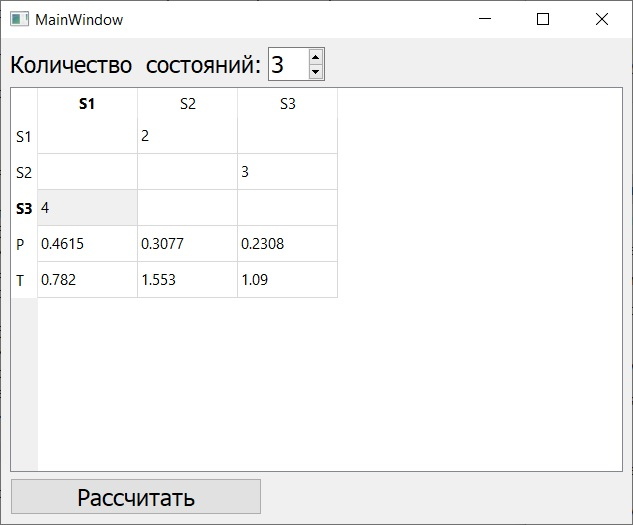
\includegraphics[scale=0.9]{source/11}}
		\centering\caption{Главное окно}
	\end{figure}

	\begin{figure}[h!]
		\centering{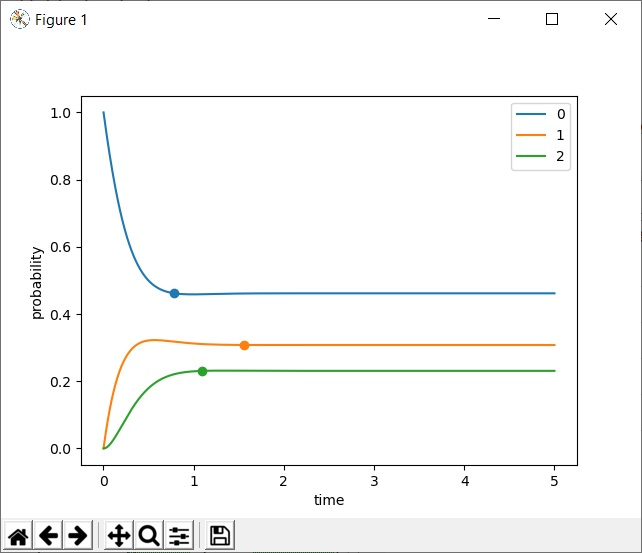
\includegraphics[scale=0.85]{source/12}}
		\centering\caption{Графики}
	\end{figure}
	\newpage
	
	\textbf{Пример 2}
	\begin{figure}[h!]
		\centering{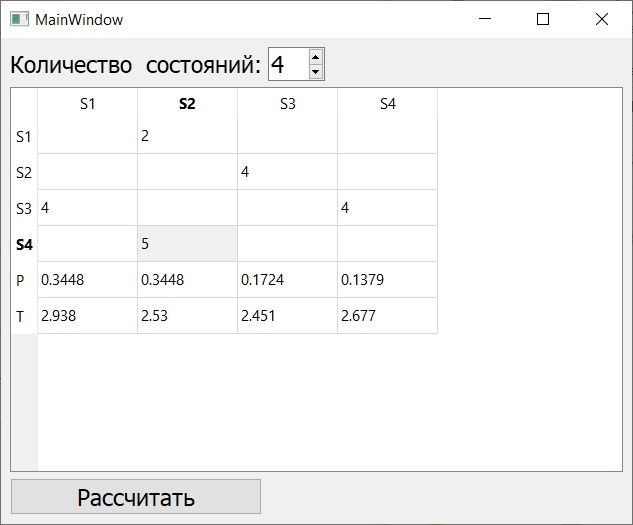
\includegraphics[scale=0.9]{source/21}}
		\centering\caption{Главное окно}
	\end{figure}
	
	\begin{figure}[h!]
		\centering{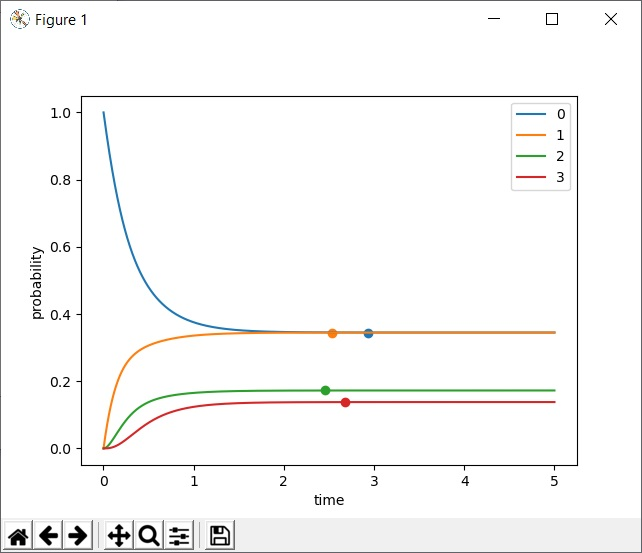
\includegraphics[scale=0.85]{source/22}}
		\centering\caption{Графики}
	\end{figure}
	\newpage
	
	\textbf{Пример 3}
	\begin{figure}[h!]
		\centering{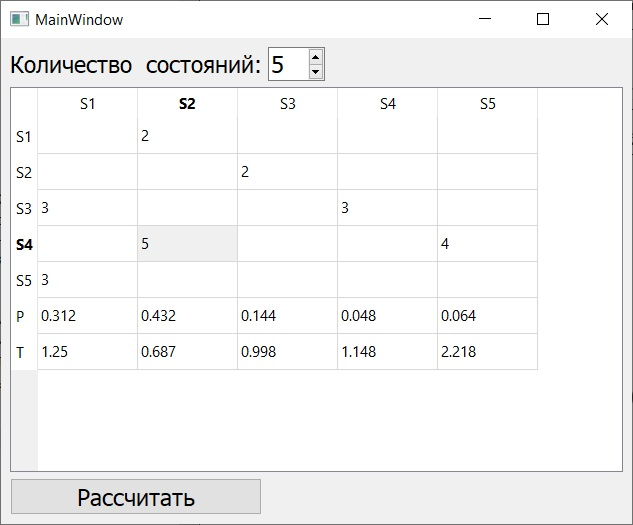
\includegraphics[scale=0.9]{source/31}}
		\centering\caption{Главное окно}
	\end{figure}
	
	\begin{figure}[h!]
		\centering{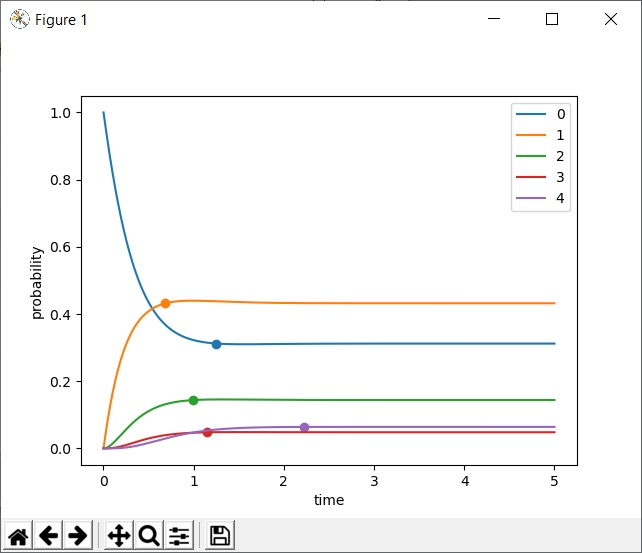
\includegraphics[scale=0.85]{source/32}}
		\centering\caption{Графики}
	\end{figure}
	
	\clearpage
	\section*{Листинги}
	\addcontentsline{toc}{section}{Листинги}
	Для запуска программы необходимо установить библиотеку PyQt5 с помощью команды: 
	pip install PyQt5
	\begin{lstlisting}[caption=main.py]
		import sys
		from PyQt5 import QtWidgets
		from PyQt5 import uic, QtWidgets, QtGui
		from PyQt5.QtWidgets import QApplication, QWidget, QListWidgetItem,  QTableWidgetItem, QMessageBox
		import design
		import solvation
		import stabilization
		import matplotlib.pyplot as plt
		
		class App(QtWidgets.QMainWindow, design.Ui_MainWindow):
			def __init__(self):
				self.is_ended = False
				self.ended_index = 0
				
				super().__init__()
				self.setupUi(self)  
				self.initUI()     
			
			def initUI(self):
				self.statesBox.valueChanged.connect(self.generateTable)
				self.table.itemChanged.connect(self.inputCheck)
				self.pushButton.clicked.connect(self.calculate)
				
				#self.setFixedSize(882, 485)
			
			def generateTable(self, value):
				self.table.setRowCount(value + 2)
				self.table.setColumnCount(value)
				self.table.clearContents()
				
				horizontalLabels = ["S" + str(i) for i in range(1, value + 1)]
				self.table.setHorizontalHeaderLabels(horizontalLabels)
				
				verticalLabels = horizontalLabels.copy()
				verticalLabels.append("P")
				verticalLabels.append("T")
				self.table.setVerticalHeaderLabels(verticalLabels)
			
			def inputCheck(self, value):
				try:
					if value.text() != "":
						float(value.text())
				except ValueError:
					QMessageBox.warning()
					value.setText("")
				
			def getMatrixFromTable(self):
				res = []
				try:
					for i in range(self.table.rowCount() - 2):
						row = []
					for j in range(self.table.columnCount()):
						item  = self.table.item(i, j)
						if item and item.text() != "":
							row.append(float(item.text()))
						else:
							row.append(0)                    
					res.append(row)
				except KeyError:
					print(res)
					QtWidgets.QMessageBox.warning()
				return res    
				
				def generateFirstProbabilities(self, count):
					res = [0] * count
					res[0] = 1
					return res
			
			def drawGraphics(self, probabilities, stabilization_time, times, probabilities_over_time):
				plt.close()
				for i in range(len(probabilities_over_time[0])):
					plt.plot(times, [j[i] for j in probabilities_over_time])
					plt.scatter(stabilization_time[i], probabilities[i])
				
				plt.legend(range(len(probabilities)))
				plt.xlabel('time')
				plt.ylabel('probability')
				plt.show()
			
			def inputProbabilities(self, probability):
				if len(probability) == 0:
					QtWidgets.QMessageBox.critical()
					return
				else:
					index = 0
					for state in probability:
						item = QTableWidgetItem()
						item.setText(str(round(state, 4)))
						self.table.setItem(self.table.rowCount() - 2, index, item)
						index += 1 
			
			def inputTimings(self, timings):
				if len(timings) == 0:
					QtWidgets.QMessageBox.critical()
					return
				else:
					index = 0
					for state in timings:
						item = QTableWidgetItem()
						item.setText(str(round(state, 4)))
						self.table.setItem(self.table.rowCount() - 1, index, item)
						index += 1 
			
			def calculate(self):
				matrix = self.getMatrixFromTable()
				probability = solvation.solve(matrix)      
				self.inputProbabilities(probability)
					
				firstProbabilities = self.generateFirstProbabilities(len(matrix))
				stabilizationTime = stabilization.CalculateStabilizationTimings(matrix, firstProbabilities, probability) 
			
				self.inputTimings(stabilizationTime)       
				times, allProbabilities = stabilization.CalculateAllProbabilities(matrix,  firstProbabilities, 5)
				self.drawGraphics(probability, stabilizationTime, times, allProbabilities)
				
		
		def main():
			app = QtWidgets.QApplication(sys.argv)
			window = App()
			window.show()
			app.exec_()
		
		if __name__ == '__main__':
			main()
	\end{lstlisting}

	\newpage
	\begin{lstlisting}[caption=stabilization.py]
		DELTA_T = 1e-3
		EPS = 1e-4
		
		def deltaPs(matrix, probabilities):
			size = len(matrix)    
			result = []
			for i in range(size):
				equations = []
				for j in range(size):
					if i == j:
						elem = probabilities[j] * (-sum(matrix[i]) + matrix[i][i])
					else:
						elem = probabilities[j] * matrix[j][i]
					equations.append(elem)
				result.append(DELTA_T * sum(equations))
			return result
		
		def CalculateStabilizationTimings(matrix, firstProbabilities, limitProbabilities):
			size = len(matrix)
			curTime = 0
			currentProbabilities = firstProbabilities.copy()
			stabilizationTimes = [0] * size
		
			while not all(stabilizationTimes):
				currdeltaPs = deltaPs(matrix, currentProbabilities)
				for i in range(size):
					if (not stabilizationTimes[i] and currdeltaPs[i] <= EPS and 
						abs(currentProbabilities[i] - limitProbabilities[i]) <= EPS):
					stabilizationTimes[i] = curTime
				currentProbabilities[i] += currdeltaPs[i]
			
			curTime += DELTA_T
			
			return stabilizationTimes
		
		def CalculateAllProbabilities(matrix, firstProbabilities, finishTime):
			size = len(matrix)
			curTime = 0
			currentProbabilities = firstProbabilities.copy()
			
			allProbabilities = []
			timings = []
			
			while curTime < finishTime:
				allProbabilities.append(currentProbabilities.copy())
				currdeltaPs = deltaPs(matrix, currentProbabilities)
				for i in range(size):
					currentProbabilities[i] += currdeltaPs[i]
				curTime += DELTA_T
				timings.append(curTime)
			
			return timings, allProbabilities
	\end{lstlisting}
	\newpage
	
	\begin{lstlisting}[caption=solvation.py]
	import numpy
	
	def coefMatrixGenerate(matrix):
		matrix = numpy.array(matrix)
		size = len(matrix)
		result = numpy.zeros((size, size))
		
		for state in range(size - 1):
			for column in range(size):
				result[state, state] -= matrix[state, column]
			for row in range(size):
				result[state, row] += matrix[row, state]
		
		for state in range(size):
			result[size - 1, state] = 1
	
	return result
	
	def createIncreaseMatrix(count):
		result = [0] * count
		result[count - 1] = 1
		return numpy.array(result)
	
	def solve(matrix):
		increaseMatrix = createIncreaseMatrix(len(matrix))
		coefMatrix = coefMatrixGenerate(matrix)
		return numpy.linalg.solve(coefMatrix, increaseMatrix)
	\end{lstlisting}
	
\end{document}